\documentclass{article}
\usepackage[utf8]{inputenc}
\usepackage[brazilian]{babel}
\usepackage{amsmath}
\usepackage{tikz}
\usepackage{enumerate}
\usepackage{enumitem}
\usepackage{amsthm,thmtools,xcolor}
\usepackage{caption}
\usepackage{float}
\usepackage[utf8]{inputenc}
\usepackage{hyperref}

\hypersetup{
    colorlinks=true,
    linkcolor=black,
    filecolor=magenta,      
    urlcolor=teal,
    pdftitle={Overleaf Example},
    pdfpagemode=FullScreen,
    }

\declaretheoremstyle[
  headfont=\color{teal}\normalfont\bfseries,
  bodyfont=\color{teal}\normalfont\itshape,
]{purple}

\declaretheorem[
  style=purple,
  name=Solução,
]{solution}

\DeclareUnicodeCharacter{2742}{\bolinha}

\newtheorem{problem}{Questão}

\title{Universidade Federal de Alagoas \\ Instituto de Computação}
\author{Monitoria de Linguagens Formais, Autômatos e Computabilidade \\ Professor Leandro Dias}
\date{Luana Júlia Nunes Ferreira, Mateus Fernando Felismino da Silva Patriota }

\begin{document}
%\setcounter{solution}{34}
\maketitle
\newpage
\tableofcontents
\newpage

%sumário
% 

\section{Linguagens Regulares}

    \subsection{Autômato Finito Determinístico}
    
    \begin{problem}
        Construa um AFD tal que $L(M) = \{ w \mid w \in \{0,1\}^*$
         e possua um número par de
        ocorrências de 0´s e de 1´s$\}$.
    \end{problem}
    
\begin{solution} Uma representação possível é:
\begin{center} 
\begin{tikzpicture}[scale=0.2]
\tikzstyle{every node}+=[inner sep=0pt]
\draw [black] (14.1,-14.9) circle (3);
\draw (14.1,-14.9) node {$q_0$};
\draw [black] (14.1,-14.9) circle (2.4);
\draw [black] (14.1,-29.3) circle (3);
\draw (14.1,-29.3) node {$q_3$};
\draw [black] (32.1,-14.9) circle (3);
\draw (32.1,-14.9) node {$q_1$};
\draw [black] (32.1,-29.3) circle (3);
\draw (32.1,-29.3) node {$q_2$};
\draw [black] (5.8,-14.9) -- (11.1,-14.9);
\fill [black] (11.1,-14.9) -- (10.3,-14.4) -- (10.3,-15.4);
\draw [black] (14.561,-17.863) arc (6.53871:-6.53871:37.203);
\fill [black] (14.56,-26.34) -- (15.15,-25.6) -- (14.16,-25.48);
\draw (15.3,-22.1) node [right] {$0$};
\draw [black] (29.142,-15.398) arc (-82.3373:-97.6627:45.314);
\fill [black] (29.14,-15.4) -- (28.28,-15.01) -- (28.42,-16);
\draw (23.1,-16.3) node [below] {$1$};
\draw [black] (17.025,-28.637) arc (100.24617:79.75383:34.153);
\fill [black] (29.18,-28.64) -- (28.48,-28) -- (28.3,-28.99);
\draw (23.1,-27.59) node [above] {$1$};
\draw [black] (31.436,-26.376) arc (-170.51122:-189.48878:25.939);
\fill [black] (31.44,-17.82) -- (30.81,-18.53) -- (31.8,-18.7);
\draw (30.58,-22.1) node [left] {$0$};
\draw [black] (29.152,-29.852) arc (-81.50267:-98.49733:40.956);
\fill [black] (17.05,-29.85) -- (17.77,-30.46) -- (17.91,-29.48);
\draw (23.1,-30.8) node [below] {$1$};
\draw [black] (17.037,-14.294) arc (99.34691:80.65309:37.328);
\fill [black] (17.04,-14.29) -- (17.91,-14.66) -- (17.75,-13.67);
\draw (23.1,-13.3) node [above] {$1$};
\draw [black] (13.321,-26.405) arc (-168.80957:-191.19043:22.184);
\fill [black] (13.32,-17.79) -- (12.68,-18.48) -- (13.66,-18.68);
\draw (12.4,-22.1) node [left] {$0$};
\draw [black] (32.697,-17.839) arc (8.5049:-8.5049:28.814);
\fill [black] (32.7,-26.36) -- (33.31,-25.64) -- (32.32,-25.5);
\draw (33.51,-22.1) node [right] {$0$};
\end{tikzpicture}
\end{center}



    \end{solution}
    
     %\begin{figure}[H]
      %      \centering
       %     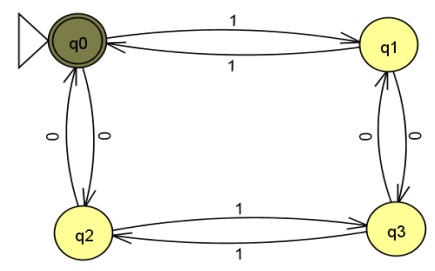
\includegraphics[scale=0.5]{solutions/q1.png}
    %\end{figure}
    
    \begin{problem}
        Construa um AFD que aceite cadeias sequenciais de "abc" em ocorrências pares.
    \end{problem}
    
    \begin{solution} O autômato pode ser representado por:
        todo
    \end{solution}
    
    \begin{problem}
        Para o autômato dado: Dê a definição formal; construa a tabela da função programa; mostre a computação da palavra 00100; que autômato é esse? Que linguagem ele reconhece?
        
        %conjunto de cadeias de 0's e 1's com número ímpar de 1‘s
\begin{center}

\begin{tikzpicture}[scale=0.2]
\tikzstyle{every node}+=[inner sep=0pt]
\draw [black] (28.1,-31.8) circle (3);
\draw (28.1,-31.8) node {$q0$};
\draw [black] (45.4,-31.8) circle (3);
\draw (45.4,-31.8) node {$q1$};
\draw [black] (45.4,-31.8) circle (2.4);
\draw [black] (43.432,-34.05) arc (-49.51444:-130.48556:10.292);
\fill [black] (30.07,-34.05) -- (30.35,-34.95) -- (31,-34.19);
\draw (36.75,-37.01) node [below] {$1$};
\draw [black] (30.266,-29.738) arc (125.83202:54.16798:11.076);
\fill [black] (43.23,-29.74) -- (42.88,-28.86) -- (42.29,-29.67);
\draw (36.75,-27.14) node [above] {$1$};
\draw [black] (48.7,-31.1) -- (48.33,-31.18);
\fill [black] (48.33,-31.18) -- (49.22,-31.5) -- (49.01,-30.52);
\draw [black] (46.628,-29.076) arc (183.47246:-104.52754:2.25);
\draw (51.17,-26.08) node [right] {$0$};
\fill [black] (48.31,-31.12) -- (49.14,-31.57) -- (49.08,-30.57);
\draw [black] (25.921,-29.755) arc (254.55605:-33.44395:2.25);
\draw (24.79,-24.96) node [above] {$0$};
\fill [black] (28.4,-28.83) -- (29.09,-28.19) -- (28.13,-27.92);
\draw [black] (22.5,-31.8) -- (25.1,-31.8);
\fill [black] (25.1,-31.8) -- (24.3,-31.3) -- (24.3,-32.3);
\end{tikzpicture}

\end{center}


    \end{problem}
    \begin{solution} Definição formal: $M = (\Sigma, Q, \delta, q_0, F)$, de modo que:
    \begin{itemize}
        \item $\Sigma = \{0,1\}$
        \item $Q = \{q_0, q_1\}$
        \item $\delta = \{\delta (q_0, 0) = q_0; \delta (q_0, 1) = q_1; \delta (q_1, 0) = q_0; \delta (q_1, 1) = q_0\}$
        \item $q_0 = q_0$
        \item $F = \{q_1\}$
    \end{itemize}
    Função computação:
    \begin{table}[H]
\centering
\begin{tabular}{|l|l|l|} 
\hline
$\delta$ & 0     & 1      \\ 
\hline
$q_0$    & $q_0$ & $q_1$  \\ 
\hline
$q_1$    & $q_1$ & $q_0$  \\
\hline
\end{tabular}
\end{table}

\noindent Computação da palavra $w = 00100$:
\begin{align*}
    \left\{\begin{matrix}
\delta^{*}(q_0,00100) & = \delta^{*}(\delta(q_0, 0),0100) & = \delta^{*}(q_0,0100) \\ 
= \delta^{*}(\delta(q_0, 0),100) & = \delta^{*}(q_0,100) & = \delta^{*}(\delta(q_0, 1),00)\\ 
= \delta^{*}(q_1,00) & = \delta^{*}(\delta(q_1, 0),0) & = \delta^{*}(q_1,0)\\ 
= \delta^{*}(\delta(q_1, 0),\epsilon) & = \delta^{*}(q_1,\epsilon) & = q_1
\end{matrix}\right.
\end{align*}
    Esse autômato é um AFD (Autômato Finito Determinístico) e reconhece as linguagens sobre o alfabeto $\{0,1\}$ que contenham um número ímpar de 1's.
    \end{solution}
    
    \begin{problem}
        Para o automato dado: Dê a definição formal; construa a tabela da função programa; mostre a computação da palavra 00100; que autômato é esse? Que linguagem ele reconhece?
        
        

\begin{center}
\begin{tikzpicture}[scale=0.2]
\tikzstyle{every node}+=[inner sep=0pt]
\draw [black] (22.9,-31.8) circle (3);
\draw (22.9,-31.8) node {$q0$};
\draw [black] (22.9,-31.8) circle (2.4);
\draw [black] (36.5,-32) circle (3);
\draw (36.5,-32) node {$q1$};
\draw [black] (47.2,-32) circle (3);
\draw (47.2,-32) node {$q2$};
\draw [black] (47.2,-45.9) circle (3);
\draw (47.2,-45.9) node {$q5$};
\draw [black] (57.9,-45.9) circle (3);
\draw (57.9,-45.9) node {$q4$};
\draw [black] (57.9,-32) circle (3);
\draw (57.9,-32) node {$q3$};
\draw [black] (33.5,-31.96) -- (25.9,-31.84);
\fill [black] (25.9,-31.84) -- (26.69,-32.36) -- (26.71,-31.36);
\draw (29.7,-32.41) node [below] {$1$};
\draw [black] (24.76,-29.471) arc (130.0693:48.24565:7.597);
\fill [black] (34.71,-29.62) -- (34.45,-28.71) -- (33.78,-29.46);
\draw (29.77,-27.17) node [above] {$0$};
\draw [black] (17.3,-31.8) -- (19.9,-31.8);
\fill [black] (19.9,-31.8) -- (19.1,-31.3) -- (19.1,-32.3);
\draw [black] (39.5,-32) -- (44.2,-32);
\fill [black] (44.2,-32) -- (43.4,-31.5) -- (43.4,-32.5);
\draw (41.85,-32.5) node [below] {$0$};
\draw [black] (44.202,-45.885) arc (-93.63969:-146.60894:25.667);
\fill [black] (24.4,-34.4) -- (24.42,-35.34) -- (25.26,-34.79);
\draw (31.95,-42.97) node [below] {$1$};
\draw [black] (54.9,-45.9) -- (50.2,-45.9);
\fill [black] (50.2,-45.9) -- (51,-46.4) -- (51,-45.4);
\draw (52.55,-45.4) node [above] {$1$};
\draw [black] (47.2,-35) -- (47.2,-42.9);
\fill [black] (47.2,-42.9) -- (47.7,-42.1) -- (46.7,-42.1);
\draw (46.7,-38.95) node [left] {$1$};
\draw [black] (57.9,-35) -- (57.9,-42.9);
\fill [black] (57.9,-42.9) -- (58.4,-42.1) -- (57.4,-42.1);
\draw (57.4,-38.95) node [left] {$1$};
\draw [black] (50.2,-32) -- (54.9,-32);
\fill [black] (54.9,-32) -- (54.1,-31.5) -- (54.1,-32.5);
\draw (52.55,-32.5) node [below] {$0$};
\end{tikzpicture}
\end{center}


    \end{problem}
    \begin{solution}
        
    \end{solution}
    \begin{problem}
        Construa um autômato que aceite aa ou bb como subpalavra. Faça a função programa.
    \end{problem}
    
    \begin{solution} O autômato pode ser representado por:
           \begin{figure}[H]
           \centering
           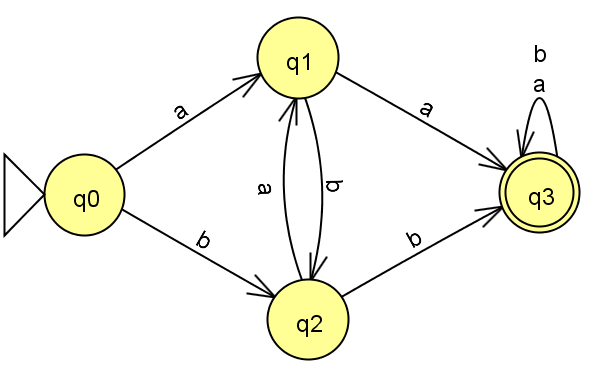
\includegraphics[scale=0.5]{solutions/q5.png}
    \end{figure}
    \end{solution}

    \subsection{Autômato Finito Não Determinístico} 
    
    \begin{problem}
        Construa um autômato que L(M) = \{ w $\mid$ w 
        possui número par de 'a' e ímpar de 'b' ou par de 'b'
        e ímpar de 'a' \}
        
    \end{problem}
    \begin{solution}
        
    \end{solution}
    \begin{problem}
        Construa um autômato que L(M) = \{ w $\mid$ w 
        o quinto símbolo da direita para a esquerda de w é 'a' \}.
        Compute a palavra 'abaaab'. Ela é aceita pelo autômato?
    \end{problem}
    \begin{solution}
        
    \end{solution}
    \begin{problem}
        Para o automato dado: Dê a definição formal; construa a tabela da função programa; mostre a computação da palavra 00100; que autômato é esse? Que linguagem ele reconhece?
        
        
\begin{center}
\begin{tikzpicture}[scale=0.2]
\tikzstyle{every node}+=[inner sep=0pt]
\draw [black] (21.8,-32) circle (3);
\draw (21.8,-32) node {$q0$};
\draw [black] (35.9,-32) circle (3);
\draw (35.9,-32) node {$q1$};
\draw [black] (48.6,-32) circle (3);
\draw (48.6,-32) node {$q2$};
\draw [black] (48.6,-32) circle (2.4);
\draw [black] (35.2,-47.2) circle (3);
\draw (35.2,-47.2) node {$q3$};
\draw [black] (16.2,-32) -- (18.8,-32);
\fill [black] (18.8,-32) -- (18,-31.5) -- (18,-32.5);
\draw [black] (38.9,-32) -- (45.6,-32);
\fill [black] (45.6,-32) -- (44.8,-31.5) -- (44.8,-32.5);
\draw (42.25,-32.5) node [below] {$1$};
\draw [black] (20.477,-29.32) arc (234:-54:2.25);
\draw (21.8,-24.75) node [above] {$1,\mbox{ }2$};
\fill [black] (23.12,-29.32) -- (24,-28.97) -- (23.19,-28.38);
\draw [black] (24.8,-32) -- (32.9,-32);
\fill [black] (32.9,-32) -- (32.1,-31.5) -- (32.1,-32.5);
\draw (28.85,-32.5) node [below] {$1$};
\draw [black] (34.577,-29.32) arc (234:-54:2.25);
\draw (35.9,-24.75) node [above] {$1,\mbox{ }2$};
\fill [black] (37.22,-29.32) -- (38.1,-28.97) -- (37.29,-28.38);
\draw [black] (48.426,-34.99) arc (-9.21275:-73.58469:14.595);
\fill [black] (48.43,-34.99) -- (47.8,-35.7) -- (48.79,-35.86);
\draw (45.51,-43.76) node [right] {$2$};
\draw [black] (33.877,-44.52) arc (234:-54:2.25);
\draw (35.2,-39.95) node [above] {$1,\mbox{ }2$};
\fill [black] (36.52,-44.52) -- (37.4,-44.17) -- (36.59,-43.58);
\draw [black] (32.209,-47.079) arc (-99.10321:-178.09934:12.677);
\fill [black] (32.21,-47.08) -- (31.5,-46.46) -- (31.34,-47.45);
\draw (24.16,-44.4) node [left] {$2$};
\end{tikzpicture}
\end{center}
    \end{problem}
    
    \begin{solution}
        Aceita cadeias $\in \{1,2\}^*$ tal que o último símbolo na cadeia tenha aparecido anteriormente
    \end{solution}
    
     \begin{problem}
        Construa um AFND tal que $L(M) = \{ w \mid w \in \{0,1\}^*
        $ e tenha dois 0’s
        consecutivos ou dois 1’s consecutivos$\}$
    \end{problem}
    
    \begin{solution} O autômato pode ser representado por:
          \begin{figure}[H]
                \centering
                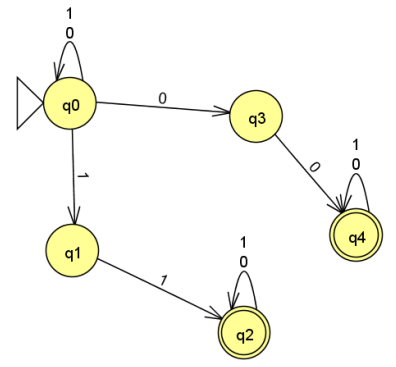
\includegraphics[scale=0.5]{solutions/q9.png}
            \end{figure}
    \end{solution}
    
    \begin{problem}
        Considerando o alfabeto $\sum = \{ a, b\}$, construa um autômato finíto não deterministico que admite cadeias em que o termo n-ésimo, a partir da direita, é b.
    \end{problem}
    
    \begin{solution} O autômato pode ser representado por:
          
\begin{center}
\begin{tikzpicture}[scale=0.2]
\tikzstyle{every node}+=[inner sep=0pt]
\draw [black] (21.8,-32) circle (3);
\draw (21.8,-32) node {$q0$};
\draw [black] (32,-32) circle (3);
\draw (32,-32) node {$q1$};
\draw [black] (43.1,-32) circle (3);
\draw (43.1,-32) node {$q2$};
\draw [black] (53.5,-32) circle (3);
\draw (53.5,-32) node {$q3$};
\draw [black] (65.6,-32) circle (3);
\draw (65.6,-32) node {$qn$};
\draw [black] (16.2,-32) -- (18.8,-32);
\fill [black] (18.8,-32) -- (18,-31.5) -- (18,-32.5);
\draw [black] (35,-32) -- (40.1,-32);
\fill [black] (40.1,-32) -- (39.3,-31.5) -- (39.3,-32.5);
\draw (37.55,-32.5) node [below] {$0,\mbox{ }1$};
\draw [black] (20.477,-29.32) arc (234:-54:2.25);
\draw (21.8,-24.75) node [above] {$0,\mbox{ }1$};
\fill [black] (23.12,-29.32) -- (24,-28.97) -- (23.19,-28.38);
\draw [black] (24.8,-32) -- (29,-32);
\fill [black] (29,-32) -- (28.2,-31.5) -- (28.2,-32.5);
\draw (26.9,-32.5) node [below] {$1$};
\draw [black] (46.1,-32) -- (50.5,-32);
\fill [black] (50.5,-32) -- (49.7,-31.5) -- (49.7,-32.5);
\draw (48.3,-32.5) node [below] {$0,\mbox{ }1$};
\draw [black] (56.5,-32) -- (62.6,-32);
\fill [black] (62.6,-32) -- (61.8,-31.5) -- (61.8,-32.5);
\draw (59.55,-32.5) node [below] {$0,\mbox{ }1$};
\end{tikzpicture}
\end{center}

    \end{solution}
    
    %\subsection{Autômato Finito com Movimentos Vazios} 
    
    \subsection{Expressão Regular}
    
    \begin{problem}
       Considerando o alfabeto $\sum = \{ a, b \}$, escreva uma expressão regular que represente a linguagem:
       \begin{enumerate}[label=(\alph*)]
           \item que começa com $b$ e termina com uma quantidade indefinida de $a$, incluindo a palavra vazia;
           \item que começa com $a$, termina com $b$ e pode conter uma infinidade de letras, exceto a palavra vazia;
           \item que tem sempre um número par de letras $a$;
           \item que possui $aa$ como subpalavra;
           \item que possui $bbb$ como sufixo;
       \end{enumerate}
    \end{problem}
    \begin{solution}
        
    \end{solution}
    \begin{problem}
       Considerando o alfabeto $\sum = \{ a, b\}$, descreva que tipo de linguagem cada expressão regular representa.
       \begin{enumerate}[label=(\alph*)]
            \item $ab^{*}$
            \item $(a+b)^{*}$
           \item $(a+b)^{*}aa(a+b)^{*}$
           \item $(a+\varepsilon )(b+ba)^{*}$
           \item $(a+b)^{*}(aa+bb)$
       \end{enumerate}
    \end{problem}
    \begin{solution}
        
    \end{solution}
    \subsection{Gramática Regular}
    
        \begin{problem}
           Dê a definição de Gramática Regular. Com isso, classifique e exemplifique os tipos de gramática regular.
        \end{problem}
        \begin{solution}
        
    \end{solution}
        \begin{problem}
           A partir da expressão regular $w = a(ba)^{*}$, determine as regras de produção de sua respectiva gramática linear à direita. Em seguida, exemplifique para a palavra $w = ababa$.
        \end{problem}
        \begin{solution}
        
    \end{solution}
        
        \begin{problem}
           A partir da expressão regular $w = 01^{*}0^{*}$, determine as regras de produção de sua respectiva gramática regular. Em seguida, exemplifique para a palavra $w = 011100$.
        \end{problem}
        \begin{solution}
        
    \end{solution}
        \begin{problem}
           A partir da expressão regular $w = (x+y)^{*}$, determine as regras de produção de sua respectiva gramática regular. Em seguida, exemplifique para a palavra $w = xyx$.
        \end{problem}
        \begin{solution}
        
    \end{solution}
        \begin{problem}
        Considerando o alfabeto $\sum = \{ 0, 1\}$, construa a gramática regular do seguinte autômato:
    
        \begin{center}
\begin{tikzpicture}[scale=0.2]
\tikzstyle{every node}+=[inner sep=0pt]
\draw [black] (21.3,-32) circle (3);
\draw (21.3,-32) node {$q0$};
\draw [black] (38.5,-32) circle (3);
\draw (38.5,-32) node {$q1$};
\draw [black] (38.5,-32) circle (2.4);
\draw [black] (58.2,-32) circle (3);
\draw (58.2,-32) node {$q2$};
\draw [black] (15.7,-32) -- (18.3,-32);
\fill [black] (18.3,-32) -- (17.5,-31.5) -- (17.5,-32.5);
\draw [black] (55.765,-33.744) arc (-60.15732:-119.84268:14.901);
\fill [black] (55.77,-33.74) -- (54.82,-33.71) -- (55.32,-34.58);
\draw (48.35,-36.22) node [below] {$1$};
\draw [black] (19.977,-29.32) arc (234:-54:2.25);
\draw (21.3,-24.75) node [above] {$0$};
\fill [black] (22.62,-29.32) -- (23.5,-28.97) -- (22.69,-28.38);
\draw [black] (24.3,-32) -- (35.5,-32);
\fill [black] (35.5,-32) -- (34.7,-31.5) -- (34.7,-32.5);
\draw (29.9,-32.5) node [below] {$1$};
\draw [black] (41.132,-30.568) arc (113.74666:66.25334:17.923);
\fill [black] (41.13,-30.57) -- (42.07,-30.7) -- (41.66,-29.79);
\draw (48.35,-28.55) node [above] {$1$};
\draw [black] (56.877,-29.32) arc (234:-54:2.25);
\draw (58.2,-24.75) node [above] {$0$};
\fill [black] (59.52,-29.32) -- (60.4,-28.97) -- (59.59,-28.38);
\draw [black] (37.177,-29.32) arc (234:-54:2.25);
\draw (38.5,-24.75) node [above] {$0$};
\fill [black] (39.82,-29.32) -- (40.7,-28.97) -- (39.89,-28.38);
\end{tikzpicture}
\end{center}


        \end{problem}
        \begin{solution}
        
    \end{solution}
         \begin{problem}
        Considerando o alfabeto $\sum = \{ 0, 1\}$, construa a gramática regular do seguinte autômato:
        
        \begin{center}
\begin{tikzpicture}[scale=0.2]
\tikzstyle{every node}+=[inner sep=0pt]
\draw [black] (21.3,-32) circle (3);
\draw (21.3,-32) node {$q0$};
\draw [black] (21.3,-32) circle (2.4);
\draw [black] (14.3,-32) -- (18.3,-32);
\fill [black] (18.3,-32) -- (17.5,-31.5) -- (17.5,-32.5);
\draw [black] (19.977,-29.32) arc (234:-54:2.25);
\draw (21.3,-24.75) node [above] {$0,\mbox{ }1$};
\fill [black] (22.62,-29.32) -- (23.5,-28.97) -- (22.69,-28.38);
\end{tikzpicture}
\end{center}

        \end{problem}
        \begin{solution}
        
    \end{solution}
         \begin{problem}
        Considerando o alfabeto $\sum = \{ 0, 1\}$, construa a gramática regular do seguinte autômato:
        
        
\begin{center}
\begin{tikzpicture}[scale=0.2]
\tikzstyle{every node}+=[inner sep=0pt]
\draw [black] (18.9,-31.2) circle (3);
\draw (18.9,-31.2) node {$q0$};
\draw [black] (18.9,-31.2) circle (2.4);
\draw [black] (39.3,-31.2) circle (3);
\draw (39.3,-31.2) node {$q1$};
\draw [black] (18.9,-48.6) circle (3);
\draw (18.9,-48.6) node {$q2$};
\draw [black] (38.4,-48.6) circle (3);
\draw (38.4,-48.6) node {$q3$};
\draw [black] (11.9,-31.2) -- (15.9,-31.2);
\fill [black] (15.9,-31.2) -- (15.1,-30.7) -- (15.1,-31.7);
\draw [black] (21.446,-29.621) arc (116.75888:63.24112:17);
\fill [black] (36.75,-29.62) -- (36.26,-28.81) -- (35.81,-29.71);
\draw (29.1,-27.3) node [above] {$1$};
\draw [black] (36.497,-32.264) arc (-72.67547:-107.32453:24.84);
\fill [black] (21.7,-32.26) -- (22.32,-32.98) -- (22.62,-32.02);
\draw (29.1,-33.89) node [below] {$1$};
\draw [black] (40.63,-33.884) arc (20.71172:-26.63359:15.194);
\fill [black] (40,-46.07) -- (40.81,-45.58) -- (39.91,-45.13);
\draw (42.17,-40.07) node [right] {$0$};
\draw [black] (37.026,-45.939) arc (-158.50563:-207.41624:14.795);
\fill [black] (37.66,-33.71) -- (36.85,-34.19) -- (37.73,-34.65);
\draw (35.44,-39.73) node [left] {$0$};
\draw [black] (35.565,-49.575) arc (-74.3756:-105.6244:25.673);
\fill [black] (21.74,-49.57) -- (22.37,-50.27) -- (22.64,-49.31);
\draw (28.65,-51.02) node [below] {$1$};
\draw [black] (21.438,-47.009) arc (116.72118:63.27882:16.039);
\fill [black] (35.86,-47.01) -- (35.37,-46.2) -- (34.92,-47.1);
\draw (28.65,-44.8) node [above] {$1$};
\draw [black] (17.303,-46.067) arc (-153.89154:-206.10846:14.015);
\fill [black] (17.3,-33.73) -- (16.5,-34.23) -- (17.4,-34.67);
\draw (15.37,-39.9) node [left] {$0$};
\draw [black] (20.576,-33.681) arc (27.63769:-27.63769:13.408);
\fill [black] (20.58,-46.12) -- (21.39,-45.64) -- (20.5,-45.18);
\draw (22.61,-39.9) node [right] {$0$};
\end{tikzpicture}
\end{center}
        \end{problem}
    \begin{solution}
        
    \end{solution}
    %\subsection{Algoritmo de Minimização}
    
    \subsection{Autômato Finito com Saída}
    
        \subsubsection{Máquina de Mealy}
            \begin{problem}
                    Dê a definição matemática de Máquina de Mealy.
            \end{problem}
            \begin{solution}
        
    \end{solution}
            \begin{problem}
                    Escreva a definição para a Máquina de Mealy a seguir e calcule a fita de saída para as fitas de entrada abaixo, caso a palavra seja aceita. Por fim, responda: que tipo de tarefa esse autômato desempenha? Dica: lógica booleana.
                    \begin{center}
\begin{tikzpicture}[scale=0.2]
\tikzstyle{every node}+=[inner sep=0pt]
\draw [black] (24.2,-24.2) circle (3);
\draw (24.2,-24.2) node {$q0$};
\draw [black] (45.3,-24.2) circle (3);
\draw (45.3,-24.2) node {$q2$};
\draw [black] (33,-41.1) circle (3);
\draw (33,-41.1) node {$q1$};
\draw [black] (25.59,-26.86) -- (31.61,-38.44);
\fill [black] (31.61,-38.44) -- (31.69,-37.5) -- (30.8,-37.96);
\draw (27.91,-33.79) node [left] {$(0,0)$};
\draw [black] (27.2,-24.2) -- (42.3,-24.2);
\fill [black] (42.3,-24.2) -- (41.5,-23.7) -- (41.5,-24.7);
\draw (34.75,-24.7) node [below] {$(1,1)$};
\draw [black] (34.77,-38.67) -- (43.53,-26.63);
\fill [black] (43.53,-26.63) -- (42.66,-26.98) -- (43.47,-27.57);
\draw (39.74,-34.03) node [right] {$(1,1)$};
\draw [black] (17.1,-24.2) -- (21.2,-24.2);
\fill [black] (21.2,-24.2) -- (20.4,-23.7) -- (20.4,-24.7);
\draw [black] (34.323,-43.78) arc (54:-234:2.25);
\draw (33,-48.35) node [below] {$(0,0)$};
\fill [black] (31.68,-43.78) -- (30.8,-44.13) -- (31.61,-44.72);
\end{tikzpicture}
\end{center}
                    \begin{enumerate}[label=(\alph*)]
                        \item 01000
                        \item 0000
                        \item 1110011
                        \item 11
                    \end{enumerate}
            
            \end{problem}
            \begin{solution}
        
    \end{solution}
            \begin{problem}
                  Transforme a Máquina de Mealy da questão anterior na sua Máquina de Moore equivalente.
            \end{problem}
            \begin{solution}
        
    \end{solution}
        \subsubsection{Máquina de Moore}
            \begin{problem}
                    Dê a definição matemática de Máquina de Moore.
            \end{problem}
            \begin{solution}
        
    \end{solution}
            \begin{problem}
                Escreva a definição para a Máquina de Moore a seguir e calcule a fita de saída para as fitas de entrada abaixo, caso a palavra seja aceita. Por fim, responda: que tipo de tarefa esse autômato desempenha? 
                 \begin{center}
\begin{tikzpicture}[scale=0.2]
\tikzstyle{every node}+=[inner sep=0pt]
\draw [black] (24.1,-24.2) circle (3);
\draw (24.1,-24.2) node {$(q0,0)$};
\draw [black] (45.3,-24.2) circle (3);
\draw (45.3,-24.2) node {$(q2,1)$};
\draw [black] (45.3,-24.2) circle (2.4);
\draw [black] (27.1,-24.2) -- (42.3,-24.2);
\fill [black] (42.3,-24.2) -- (41.5,-23.7) -- (41.5,-24.7);
\draw (34.7,-24.7) node [below] {$b$};
\draw [black] (17,-24.2) -- (21.1,-24.2);
\fill [black] (21.1,-24.2) -- (20.3,-23.7) -- (20.3,-24.7);
\draw [black] (25.423,-26.88) arc (54:-234:2.25);
\draw (24.1,-31.45) node [below] {$a$};
\fill [black] (22.78,-26.88) -- (21.9,-27.23) -- (22.71,-27.82);
\end{tikzpicture}
\end{center}
                \begin{enumerate}[label=(\alph*)]
                        \item aaab
                        \item abab
                        \item aa
                    \end{enumerate}
                 
            \end{problem}
            \begin{solution}
        
    \end{solution}
            \begin{problem}
                  Transforme a Máquina de Moore da questão anterior na sua Máquina de Mealy equivalente.
            \end{problem}
            \begin{solution}
        
    \end{solution}
    \subsection{Conversão de AFND para AFD}

    \begin{problem}
                O que este autômato faz? Compute w = 'baaa' e converta para AFD.
                  \begin{figure}[!htb]
                      \centering
                      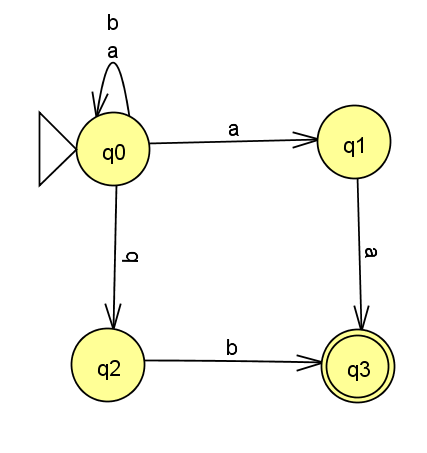
\includegraphics[scale=0.5]{aabbsulfixo.png}
                  \end{figure}
    \end{problem}
    \begin{solution}
        
    \end{solution}
     \begin{problem}
         O que este autômato faz? Compute w = 'baba' e 
         converta para AFD.
                \begin{figure}[!htb]
                    \centering
                    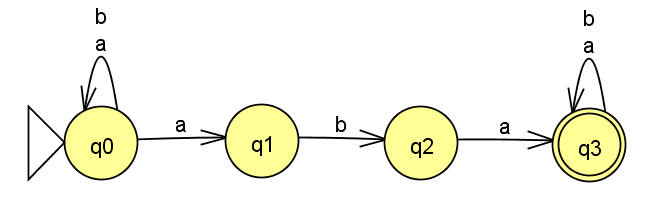
\includegraphics[scale=0.5]{abasubpalavra.png}
                \end{figure}
    \end{problem}
\begin{solution}
        
    \end{solution}
\section{Linguagens Livres de Contexto}

    \subsection{Autômato com Pilha}
    
    \begin{problem}
         Construa um autômato tal que $L(M) = \{ wcw^r \mid w \in \{0,1\}^*\}$. Na prática, o que esse autômato reconhece?
    \end{problem}
    \begin{solution}
        
    \end{solution}
    \begin{problem}
         Construa um autômato tal que $L(M) = \{ a^n b^m b^c (c = n + m)\mid n>=0$, $m>=0 \in \{a,b\}^*\}$. Exemplo de palavra reconhecida $a^1 b^1 b^2 = abbb$.
    \end{problem}
    \begin{solution}
        
    \end{solution}
    \subsection{Árvore de Derivação}
    
    \begin{problem}
         Construa a árvore de derivalção da palavra W = x+x*[x-x] $G = \{ \{E\},\{+,-,*,[.],x\},P,E\}$ e $P = \{ E -> E+E | E*E | [E] , x\}$.  
    \end{problem}
    \begin{solution}
        
    \end{solution}
    \begin{problem}
         A palavra gerada pela árvore é ambigua? Por quê? Se sim, gera a palavra de outra forma diferente da anterir.  
    \end{problem}
\begin{solution}
        
    \end{solution}
\section{Linguagens Enumeradas e Recursivamente e Sensíveis ao Contexto}

    \subsection{Máquina de Turing}
        \begin{problem}
                Defina formalmente a Máquina de Turing; contrua um autômato de exemplo e, em seguida, compute uma palavra de sua escolha.
        \end{problem}
        \begin{solution}
        
    \end{solution}
    \subsection{Hipótese de Church}
        \begin{problem}
              Descreva a hipótese Church-Turing.
        \end{problem}
        \begin{solution}
        
    \end{solution}
\section{Computabilidade}

    \subsection{Cálculo Lambda}
    \begin{problem}
        Reduza as expressões a seguir:
        \begin{enumerate}[label=(\alph*)]
            \item ($\lambda$ x.2*x + 1) 3
            \item (($\lambda x.(\lambda y.x-y) 2 ) -1$
            \item (($\lambda$ x.$\lambda$y. – x y) 9 ) 4
        \end{enumerate}
    \end{problem}
    
    \begin{solution} Reduções:
        \begin{enumerate}[label=(\alph*)]
            \item $(\lambda x. 2*x + 1) 3 = 2*3 + 1 = 7$
            \item (($\lambda x.(\lambda y.x-y) 2 ) -1) = (\lambda y.-1-y) 2  = -1-2 = -3$
            \item $((\lambda x. \lambda y. – x y) 9 ) 4 =  \lambda y. – 4 y) 9 = -4*9 = -36 $
        \end{enumerate}
    \end{solution}

\section{Atividades 2020.1}
\subsection{Atividade 1}
\begin{problem} Estudar autômatos finitos determinísticos.
Algumas sugestões de materiais auxiliares:
\begin{itemize}
    \item \url{http://eaulas.usp.br/portal/video.action?idItem=17133}
    \item \url{https://www.cin.ufpe.br/~gcb/tc/tc_automato_finitos.pdf}
    \item \url{http://www2.fct.unesp.br/docentes/dmec/olivete/lfa/arquivos/Apostila.pdf}  (página 77)
\end{itemize}

\end{problem}
\begin{solution} Leitura a cargo do(a) estudante.
\end{solution}

\subsection{Atividade 2}
\begin{problem} Faça o Autômato Finito Determinístico (AFD) que aceita a linguagem que contém palavras com sufixo "01".
\end{problem}

\begin{solution}
    O autômato pode ser representado por:

\begin{figure}[H]
        \centering
        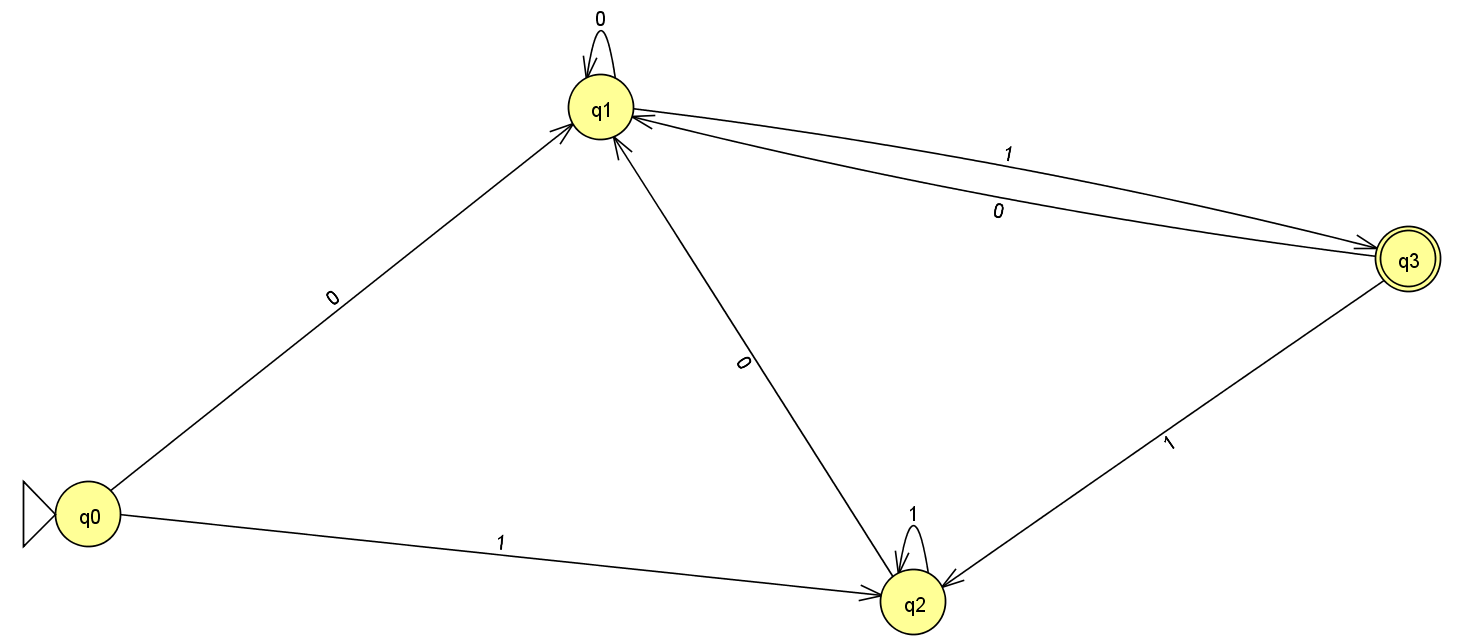
\includegraphics[scale=0.3]{figs/atividades/a2q1.png}
\end{figure}
\end{solution}


\begin{problem}
     Faça o problema anterior com o Autômato Finito Não Determinístico (AFN).
\end{problem}

\begin{solution}
    O autômato pode ser representado por:

\begin{figure}[H]
        \centering
        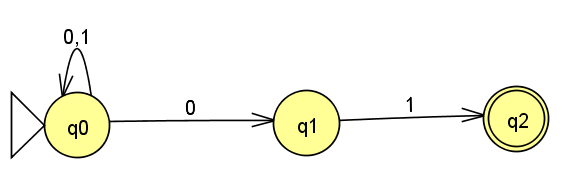
\includegraphics[scale=0.45]{figs/atividades/a2q2.png}
\end{figure}
\end{solution}

\begin{problem} Converta, manualmente, o autômato AFN da questão anterior no AFD, sem usar o JFLAP (você pode usar o JFLAP para comparar com sua resposta).
\end{problem}

\begin{solution}
    TODO
\end{solution}
\subsection{Atividade 3}
\begin{problem} Defina a expressão regular que denota todas as cadeias de 0's e 1's com ao menos dois 0's consecutivos.
\end{problem}

\begin{solution}
    A Expressão regular é dada por ER = $(0 + 1)^*00(0 + 1)^*$
\end{solution}

\begin{problem} Faça o autômato finito equivalente ao exercício 1 acima.
\end{problem}

\begin{solution}
Podemos subdividir o autômato em $r1 = 0; r2 = 1; r3 = (0 + 1)^*; r4 = (0 + 1)^*00^*(0 + 1)^* = r3r1r1r3;$ Logo, o autômato será definido por:
    \begin{figure}[H]
        \centering
        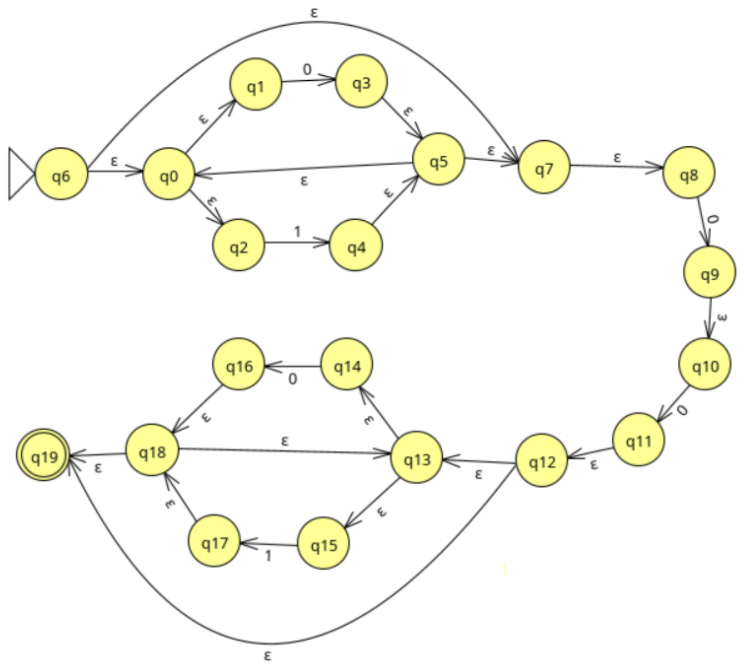
\includegraphics[scale=0.45]{figs/atividades/a3q2.png}
    \end{figure}
\end{solution}

\begin{problem} Defina a gramática regular para a linguagem sobre o alfabeto $\{0,1\}$, $L = \{w\in \Sigma^{*} | w$ tem no máximo tamanho $3\}$.
\end{problem}

\begin{solution}
     Definindo a gramática G = (V, T, P, S). Tal que:
 
\begin{enumerate}[label=]
    \item $V = \{A,B\};$
    \item $T = \{0, 1\};$
    \item $P = \{S \rightarrow 0A | 1A | \epsilon; A \rightarrow 0B | 1B | \epsilon; B \rightarrow 0 | 1 | \epsilon \};$
\end{enumerate}
\end{solution}

\begin{problem} Construa o autômato equivalente ao exercício acima.
\end{problem}

\begin{solution}
O autômato equivalente é dado por:
\begin{center}
\begin{tikzpicture}[scale=0.2]
\tikzstyle{every node}+=[inner sep=0pt]
\draw [black] (13.3,-14.9) circle (3);
\draw (13.3,-14.9) node {$q_0$};
\draw [black] (26,-14.9) circle (3);
\draw (26,-14.9) node {$q_1$};
\draw [black] (37.9,-14.9) circle (3);
\draw (37.9,-14.9) node {$q_3$};
\draw [black] (37.9,-14.9) circle (2.4);
\draw [black] (26,-26.5) circle (3);
\draw (26,-26.5) node {$q_2$};
\draw [black] (5,-14.9) -- (10.3,-14.9);
\fill [black] (10.3,-14.9) -- (9.5,-14.4) -- (9.5,-15.4);
\draw [black] (29,-14.9) -- (34.9,-14.9);
\fill [black] (34.9,-14.9) -- (34.1,-14.4) -- (34.1,-15.4);
\draw (31.95,-15.4) node [below] {$\epsilon$};
\draw [black] (16.3,-14.9) -- (23,-14.9);
\fill [black] (23,-14.9) -- (22.2,-14.4) -- (22.2,-15.4);
\draw (19.65,-15.4) node [below] {$0,1$};
\draw [black] (15.671,-13.067) arc (122.99947:57.00053:18.231);
\fill [black] (35.53,-13.07) -- (35.13,-12.21) -- (34.59,-13.05);
\draw (25.6,-9.63) node [above] {$\epsilon$};
\draw [black] (26,-17.9) -- (26,-23.5);
\fill [black] (26,-23.5) -- (26.5,-22.7) -- (25.5,-22.7);
\draw (25.5,-20.7) node [left] {$0,1$};
\draw [black] (28.15,-24.41) -- (35.75,-16.99);
\fill [black] (35.75,-16.99) -- (34.83,-17.19) -- (35.53,-17.91);
\draw (34.39,-21.18) node [below] {$0,1,\epsilon$};
\end{tikzpicture}
\end{center}



\end{solution}

\begin{problem} Construa o AFN com movimentos vazios, com alfabeto $\{0,1\}$, que reconheça a linguagem que tenha números pares de 0's ou de 1's.
\end{problem}

\begin{solution}
O AFN pode ser representado por:
    \begin{figure}[H]
        \centering
        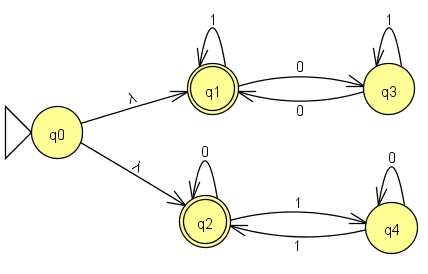
\includegraphics[scale=0.6]{figs/atividades/a3q5.png}
    \end{figure}
\end{solution}


\subsection{Atividade 4}
\begin{problem} Defina a gramática livre de contexto que gere palíndromos. Supondo o alfabeto $\{a,b\}$, mostre a derivação de uma palavra. Ex.: aba
\end{problem}

\begin{solution}
 Definindo a gramática G = (V, T, P, S). Tal que:
 
\begin{enumerate}[label=]
    \item $V = \{S\};$
    \item $T = \{a, b\};$
    \item $P = \{S \rightarrow \epsilon; S \rightarrow a; S \rightarrow  b; S \rightarrow aSa; S \rightarrow bSb\};$
\end{enumerate}

\end{solution}
\begin{problem} Faça o autômato com pilha que reconheça a linguagem $L=wcwR, w \in \{a,b\}^{*}$ (R significa reversa). Ex.: abcba.
\end{problem}
\begin{solution}
O autômato com pilha pode ser representado por:
\begin{figure}[H]
        \centering
        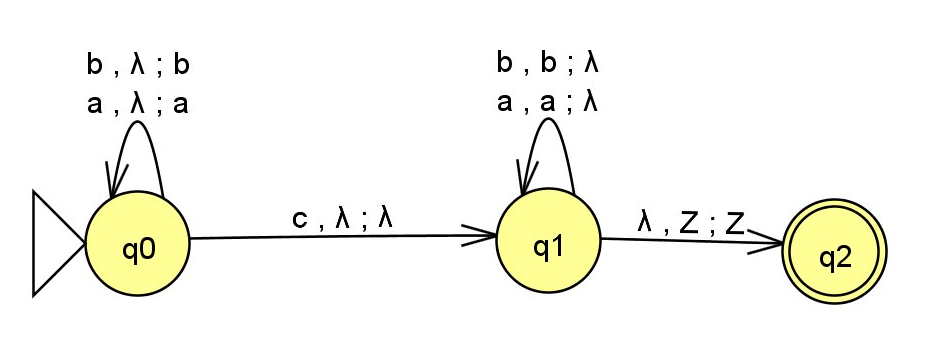
\includegraphics[scale=0.45]{figs/atividades/a4q2.png}
\end{figure}


\end{solution}

\subsection{Atividade 5} 
\begin{problem} Faça a máquina de Turing com alfabeto $\Sigma =\{a,b\}$ que remova os símbolos $b$ da entrada. Exemplo:
$ababa \rightarrow aaa$ (sem brancos/vazios, somente a's).
\end{problem}
\begin{solution} A máquina de Turing que resolve o problema pode ser representada por:
\begin{figure}[H]
        \centering
        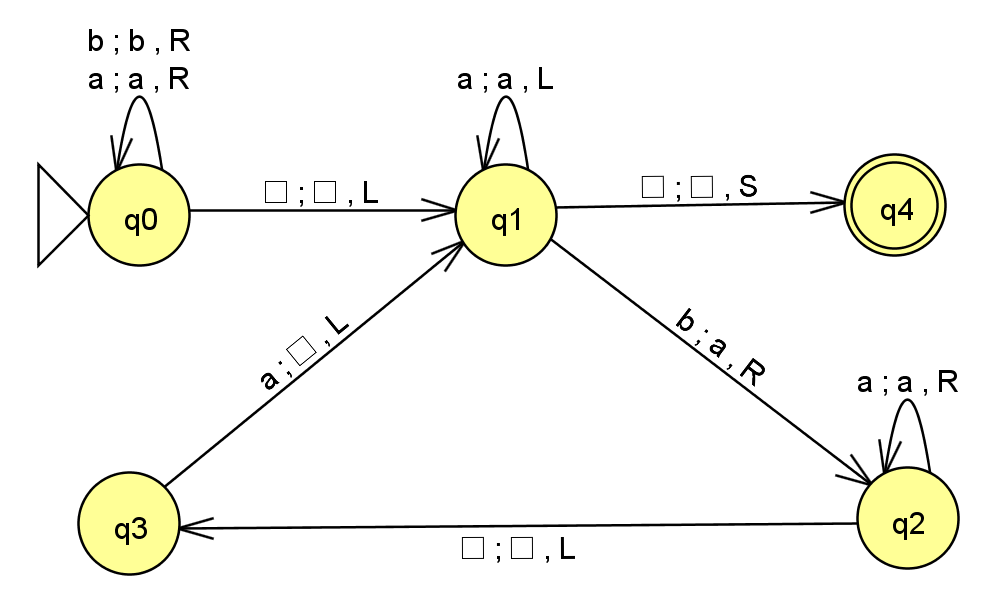
\includegraphics[scale=0.45]{figs/atividades/a5q1.png}
\end{figure}

\end{solution}

\begin{problem} Faça a máquina de Turing para inverter os bits de uma entrada binária, ou seja, alfabeto ${0,1}$. Exemplo:
$[0001011] \rightarrow [1110100]$.
\end{problem}

\begin{solution} A máquina de Turing para inverter os bits de uma entrada binária é representada por:

\begin{figure}[H]
        \centering
        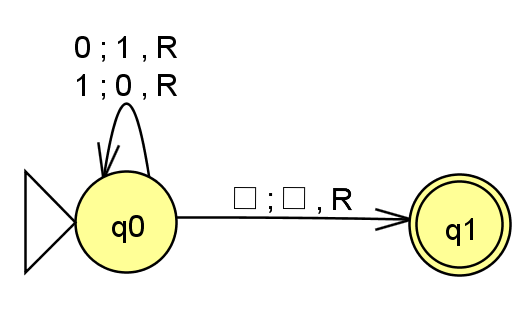
\includegraphics[scale=0.45]{figs/atividades/a5q2.png}
\end{figure}

\end{solution}


\subsection{Atividade 6}
\begin{problem} Suponha as funções constzero (número zero) , antecessor, id (identidade), $proj^{3}_{3}$ (projeção), a
função subtração sub: $N_2 \rightarrow N$ pode ser definida usando recursão primitiva:
\begin{itemize}
    \item sub(x,0) = id(x)
    \item sub(x, y + 1) = antecessor o $proj^{3}_{3}$(x, y, sub(x, y))
\end{itemize}
Determine o valor de sub(2, 3)
\end{problem}
\begin{solution}
Desenvolvendo as funções, temos:

sub(2,3) = antecessor $\circ$ $proj^{3}_{3}$(2, 2, sub(2, 2))\\
= antecessor $\circ$ $proj^{3}_{3}$(2,2, antecessor $\circ$ $proj^{3}_{3}$(2,1, sub(2,1))))\\
= antecessor $\circ$ $proj^{3}_{3}$(2,2, antecessor $\circ$ $proj^{3}_{3}$(2,1, antecessor $\circ$ $proj^{3}_{3}$(2,0, sub(2,0))))\\
= antecessor $\circ$ $proj^{3}_{3}$(2,2, antecessor $\circ$ $proj^{3}_{3}$(2,1, antecessor $\circ$ $proj^{3}_{3}$(2,0, id(2))))\\
= antecessor $\circ$ $proj^{3}_{3}$(2,2, antecessor $\circ$ $proj^{3}_{3}$(2,1, antecessor $\circ$ $proj^{3}_{3}$(2,0,2)))\\
= antecessor $\circ$ $proj^{3}_{3}$(2,2, antecessor $\circ$ $proj^{3}_{3}$(2,1, antecessor(2)))\\
= antecessor $\circ$ $proj^{3}_{3}$(2,2, antecessor $\circ$ $proj^{3}_{3}$(2,1, 1))\\
= antecessor $\circ$ $proj^{3}_{3}$(2,2, antecessor(1))\\
= antecessor $\circ$ $proj^{3}_{3}$(2,2,0)\\
= antecessor(0)\\
= 0\\
\end{solution}


\subsection{Atividade 7}
\begin{problem} Faça as seguintes reduções:
     \begin{itemize}
         \item $((\lambda n.2n) 7)$
         \item $(\lambda x.(x^2 - 2x+5)) 2$
         \item $(\lambda x.((\lambda y.(xy)) a)) b$
         \item $(\lambda x.(\lambda y.(xy))) (\lambda y.x)$
     \end{itemize}
\end{problem}
\begin{solution} Reduções:
    \begin{itemize}
         \item $((\lambda n.2n) 7) = (2*7) = 14$
         \item $(\lambda x.(x^2 - 2x+5)) 2 = (2^2 - 2*2 +5) = 5$
         \item $(\lambda x.((\lambda y.(xy)) a)) b = ((\lambda y.(by)) a) = ba$
         \item $(\lambda x.(\lambda y.(xy))) (\lambda y.x) = \lambda y. (\lambda y. x y) = \lambda y. x$
     \end{itemize}
\end{solution}

\subsection{Atividade 8}
\begin{problem} Explique com suas palavras o que você entende por computabilidade.
\end{problem}

\begin{solution}
Computabilidade está relacionada ao estudo de problemas e à resolução destes através de dado algoritmo em tempo determinado.
\end{solution}

\begin{problem} Explique com suas palavras o que você entende por princípio da redução.
\end{problem}

\begin{solution}
O princípio da redução é uma forma de solucionar problemas utilizando recursividade. Ou seja, é realizado a divisão de um problema menores partes, até que cada um desses pequenos pedaços/problemas possua uma solução conhecida.
\end{solution}

\section{Avaliações Anteriores}
    \subsection{Avaliação 01 - 2020.1}

\begin{problem} Que tipo de autômato é ilustrado na figura abaixo? Que linguagem ele reconhece? Mostre a
definição formal. Mostre a computação da palavra $w=0111$. A palavra é aceita?
\begin{center}
\begin{tikzpicture}[scale=0.2]
\tikzstyle{every node}+=[inner sep=0pt]
\draw [black] (24.6,-15) circle (3);
\draw (24.6,-15) node {$q_0$};
\draw [black] (37,-8.2) circle (3);
\draw (37,-8.2) node {$q_1$};
\draw [black] (37,-8.2) circle (2.4);
\draw [black] (36.4,-21.5) circle (3);
\draw (36.4,-21.5) node {$q_2$};
\draw [black] (37.723,-24.18) arc (54:-234:2.25);
\draw (36.4,-28.75) node [below] {$1$};
\fill [black] (35.08,-24.18) -- (34.2,-24.53) -- (35.01,-25.12);
\draw [black] (16.3,-15) -- (21.6,-15);
\fill [black] (21.6,-15) -- (20.8,-14.5) -- (20.8,-15.5);
\draw [black] (23.277,-12.32) arc (234:-54:2.25);
\draw (24.6,-7.75) node [above] {$0$};
\fill [black] (25.92,-12.32) -- (26.8,-11.97) -- (25.99,-11.38);
\draw [black] (27.23,-16.45) -- (33.77,-20.05);
\fill [black] (33.77,-20.05) -- (33.31,-19.23) -- (32.83,-20.1);
\draw (29.5,-18.75) node [below] {$1$};
\draw [black] (27.23,-13.56) -- (34.37,-9.64);
\fill [black] (34.37,-9.64) -- (33.43,-9.59) -- (33.91,-10.47);
\draw (31.72,-12.1) node [below] {$\epsilon$};
\draw [black] (36.54,-18.5) -- (36.86,-11.2);
\fill [black] (36.86,-11.2) -- (36.33,-11.97) -- (37.33,-12.02);
\draw (37.27,-14.87) node [right] {$1$};
\end{tikzpicture}
\end{center}
\end{problem}

\begin{solution} O autômato ilustrado nessa figura é um autômato não-determinístico com movimentos vazios. Esse autômato reconhece as seguintes linguagens: palavras vazias, palavras com sufixo $11$ e prefixo ou $0$ ou vazio. Além disso, nunca haverá $0$ precedido de $1$.
\begin{itemize}
    \item Definição formal: $M = (\{0,1\}, \{q_0, q_1, q_2\}, \delta, q_0, \{q_1\})$
    \item Computação vazia da palavra $w = 0111$:
    \begin{itemize}
        \item $\delta^{*}(\{q_0\},0111) = \delta_{\epsilon}(\{ r | r \in \delta(s, 1)$ e $s \in \delta*(\{ q_0 \}, 011)\})$
        \item $\delta^{*}(\{q_0\},011) = \delta_{\epsilon}(\{ r | r \in \delta(s, 1)$ e $s \in \delta*(\{ q_0 \}, 01)\})$
        \item $\delta^{*}(\{q_0\},01) = \delta_{\epsilon}(\{ r | r \in \delta(s, 1)$ e $s \in \delta*(\{ q_0 \}, 0)\})$
        \item $\delta^{*}(\{q_0\},0) = \delta_{\epsilon}(\{ r | r \in \delta(s, 0)$ e $s \in \delta*(\{ q_0 \}, \epsilon)\})$
    \end{itemize}
    \item Sabendo que:
    \begin{itemize}
        \item $\delta^{*}(\{q_0\},\epsilon) = \delta_{\epsilon}(\{q_0\}) = \{q_0, q_1\}$
        \item $\delta^{*}(\{q_0\},0) = \{q_0, q_1\}$
        \item $\delta^{*}(\{q_0\},01) = \{q_0, q_2\}$
        \item $\delta^{*}(\{q_0\},011) = \{q_1, q_2\}$
    \end{itemize}
    \item A computação da palavra $0111$ é $\delta^{*}(\{q_0\},0111) = \{q_1, q_2\}$ e a palavra é aceita.
\end{itemize}
\end{solution}
    
\begin{problem} Construa o autômato finito não determinístico equivalente ao da figura acima (questão anterior). Mostre os passos da
conversão.
\end{problem}    

\begin{solution} 
A máquina de estados é: $M_2 = (\{0,1\}, \{q_0,q_1,q_2\}, \delta_3, q_0, \{q_1\})$. A função computação pode ser representada da seguinte forma:
\begin{figure}[H]
    \centering
    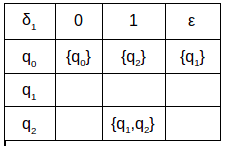
\includegraphics[scale=0.5]{figs/prova 1/tabelinha1.png}
    %\caption{Caption}
    %\label{fig:my_label}
\end{figure}
\noindent Daí, $M_3=M_{2n} = (\{0,1\},\{q_0,q_1,q_2\}, \delta_{2n}, q_0, F_n)$. A computação da palavra vazia é $F_n = \{q_0,q_1,q_2\}$.
\begin{itemize}
    \item $\delta_{\epsilon}(q_0) = \{q_0,q_1\}$
    \item $\delta_{\epsilon}(q_1) = \{q_1\}$
    \item $\delta_{\epsilon}(q_2) = \{q_2\}$
\end{itemize}
Função $\delta_n$:
\begin{itemize}
    \item $\delta_n(\{q_0\}, \epsilon) = \{q_0, q_1\}$
    \item $\delta_n(\{q_1\}, \epsilon) = \{q_1\}$ 
    \item $\delta_n(\{q_2\}, \epsilon) = \{q_2\}$
\end{itemize}
Computação:
\begin{itemize}
    \item $\delta_n(q0, 0) = \delta_3(\{q_0\}, 0) = \delta_{\epsilon}(\{ r | r \in \delta(s, 0)$ e $s \in \delta(\{ q_0 \}, \epsilon)\}) = \{q_0, q_1\}$
\item $\delta_n(q_0, 1) = \delta_3(\{q_0\}, 1) = \delta_{\epsilon}(\{ r | r \in \delta(s, 1)$ e $s \in \delta(\{ q_0 \}, \epsilon)\}) = \{q_2\}$
\item $\delta_n(q_1, 0) = \delta_3(\{q_1\}, 0) = \delta_{\epsilon}(\{ r | r \in \delta(s, 0)$ e $s \in \delta(\{ q_1 \}, \epsilon)\}) =$ indefinido
\item $\delta_n(q_1, 1) = \delta_3(\{q_1\}, 1) = \delta_{\epsilon}(\{ r | r \in \delta(s, 1)$ e $s \in \delta(\{ q_1 \}, \epsilon)\}) =$ indefinido
\item $\delta_n(q_2, 0) = \delta_3(\{q_2\}, 0) = \delta_{\epsilon}(\{ r | r \in \delta(s, 0)$ e $s \in \delta(\{ q_2 \}, \epsilon)\}) =$ indefinido
\item $\delta_n(q_2, 1) = \delta_3(\{q_2\}, 1) = \delta_{\epsilon}(\{ r | r \in \epsilon(s, 1)$ e $s \in \delta*(\{ q_2 \}, \epsilon)\}) = \{q_1, q_2\}$
\end{itemize}
Função computação:
\begin{figure}[H]
    \centering
    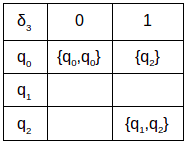
\includegraphics[scale=0.5]{figs/tabelissima.png}
    %\caption{Caption}
    %\label{fig:my_label}
\end{figure}
Representação do autômato:
\begin{center}
\begin{tikzpicture}[scale=0.2]
\tikzstyle{every node}+=[inner sep=0pt]
\draw [black] (24.6,-15) circle (3);
\draw (24.6,-15) node {$q_0$};
\draw [black] (24.6,-15) circle (2.4);
\draw [black] (38.2,-6.6) circle (3);
\draw (38.2,-6.6) node {$q_1$};
\draw [black] (38.2,-6.6) circle (2.4);
\draw [black] (52.6,-15) circle (3);
\draw (52.6,-15) node {$q_2$};
\draw [black] (51.277,-12.32) arc (234:-54:2.25);
\draw (52.6,-7.75) node [above] {$1$};
\fill [black] (53.92,-12.32) -- (54.8,-11.97) -- (53.99,-11.38);
\draw [black] (16.3,-15) -- (21.6,-15);
\fill [black] (21.6,-15) -- (20.8,-14.5) -- (20.8,-15.5);
\draw [black] (23.277,-12.32) arc (234:-54:2.25);
\draw (24.6,-7.75) node [above] {$0$};
\fill [black] (25.92,-12.32) -- (26.8,-11.97) -- (25.99,-11.38);
\draw [black] (27.6,-15) -- (49.6,-15);
\fill [black] (49.6,-15) -- (48.8,-14.5) -- (48.8,-15.5);
\draw (38.6,-15.5) node [below] {$1$};
\draw [black] (27.15,-13.42) -- (35.65,-8.18);
\fill [black] (35.65,-8.18) -- (34.7,-8.17) -- (35.23,-9.02);
\draw (32.4,-11.3) node [below] {$0$};
\draw [black] (50.01,-13.49) -- (40.79,-8.11);
\fill [black] (40.79,-8.11) -- (41.23,-8.95) -- (41.73,-8.08);
\draw (46.4,-10.3) node [above] {$1$};
\end{tikzpicture}
\end{center}
\end{solution}

\begin{problem} Construa o autômato finito, definição formal e o diagrama, com $\Sigma=\{0,1\}$, que aceita palavras
que tem 1 na quarta posição da direita para a esquerda da palavra.
\end{problem}

\begin{solution} Representação do autômato:
\begin{center}
\begin{tikzpicture}[scale=0.2]
\tikzstyle{every node}+=[inner sep=0pt]
\draw [black] (18.7,-15.7) circle (3);
\draw (18.7,-15.7) node {$q_0$};
\draw [black] (18.7,-15.7) circle (2.4);
\draw [black] (31.6,-15.7) circle (3);
\draw (31.6,-15.7) node {$q_1$};
\draw [black] (43.4,-15.7) circle (3);
\draw (43.4,-15.7) node {$q_2$};
\draw [black] (54.5,-15.7) circle (3);
\draw (54.5,-15.7) node {$q_3$};
\draw [black] (65.7,-15.7) circle (3);
\draw (65.7,-15.7) node {$q_4$};
\draw [black] (65.7,-15.7) circle (2.4);
\draw [black] (10.4,-15.7) -- (15.7,-15.7);
\fill [black] (15.7,-15.7) -- (14.9,-15.2) -- (14.9,-16.2);
\draw [black] (17.377,-13.02) arc (234:-54:2.25);
\draw (18.7,-8.45) node [above] {$0$};
\fill [black] (20.02,-13.02) -- (20.9,-12.67) -- (20.09,-12.08);
\draw [black] (21.7,-15.7) -- (28.6,-15.7);
\fill [black] (28.6,-15.7) -- (27.8,-15.2) -- (27.8,-16.2);
\draw (25.15,-16.2) node [below] {$1$};
\draw [black] (40.895,-17.323) arc (-66.9709:-113.0291:8.677);
\fill [black] (40.89,-17.32) -- (39.96,-17.18) -- (40.35,-18.1);
\draw (37.5,-18.51) node [below] {$0$};
\draw [black] (52.123,-17.497) arc (-64.54544:-115.45456:7.384);
\fill [black] (52.12,-17.5) -- (51.19,-17.39) -- (51.62,-18.29);
\draw (48.95,-18.71) node [below] {$0$};
\draw [black] (62.968,-16.914) arc (-74.20249:-105.79751:10.534);
\fill [black] (62.97,-16.91) -- (62.06,-16.65) -- (62.33,-17.61);
\draw (60.1,-17.81) node [below] {$0$};
\draw [black] (34.109,-14.083) arc (112.93153:67.06847:8.703);
\fill [black] (40.89,-14.08) -- (40.35,-13.31) -- (39.96,-14.23);
\draw (37.5,-12.89) node [above] {$1$};
\draw [black] (20.023,-18.38) arc (54:-234:2.25);
\draw (18.7,-22.95) node [below] {$1$};
\fill [black] (17.38,-18.38) -- (16.5,-18.73) -- (17.31,-19.32);
\draw [black] (45.979,-14.197) arc (110.22878:69.77122:8.593);
\fill [black] (51.92,-14.2) -- (51.34,-13.45) -- (51,-14.39);
\draw (48.95,-13.17) node [above] {$1$};
\draw [black] (57.044,-14.14) arc (111.30252:68.69748:8.412);
\fill [black] (63.16,-14.14) -- (62.59,-13.38) -- (62.23,-14.32);
\draw (60.1,-13.07) node [above] {$1$};
\end{tikzpicture}
\end{center}
Função Computação:
\begin{figure}[H]
    \centering
    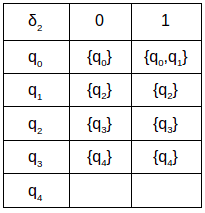
\includegraphics[scale=0.5]{figs/tabelona.png}
    %\caption{Caption}
    %\label{fig:my_label}
\end{figure}
Definição formal:
$M_2 = (\{0,1\}, \{q_0,q_1,q_2,q_3,q_4,q_5\}, \delta_2, q_0, \{q_5\})$
\end{solution}

\begin{problem} Construa o autômato finito, com alfabeto $\Sigma=\{a,b\}$, que reconheça a linguagem em que qualquer
ocorrência de b é imediatamente sucedida por a.
\end{problem}

\begin{solution} Função computação:
\begin{figure}[H]
    \centering
    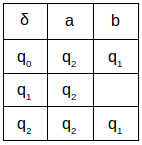
\includegraphics[scale=0.5]{figs/tabelesco.png}
    %\caption{Caption}
    %\label{fig:my_label}
\end{figure}
Representação do autômato:
\begin{center}
\begin{tikzpicture}[scale=0.2]
\tikzstyle{every node}+=[inner sep=0pt]
\draw [black] (21,-15.7) circle (3);
\draw (21,-15.7) node {$q_0$};
\draw [black] (30.9,-4.7) circle (3);
\draw (30.9,-4.7) node {$q_1$};
\draw [black] (43.4,-15.7) circle (3);
\draw (43.4,-15.7) node {$q_2$};
\draw [black] (43.4,-15.7) circle (2.4);
\draw [black] (12.7,-15.7) -- (18,-15.7);
\fill [black] (18,-15.7) -- (17.2,-15.2) -- (17.2,-16.2);
\draw [black] (23.01,-13.47) -- (28.89,-6.93);
\fill [black] (28.89,-6.93) -- (27.99,-7.19) -- (28.73,-7.86);
\draw (26.49,-11.66) node [right] {$b$};
\draw [black] (33.784,-5.511) arc (68.98951:28.31494:16.185);
\fill [black] (42.23,-12.94) -- (42.29,-12) -- (41.41,-12.48);
\draw (39.63,-7.98) node [above] {$a$};
\draw [black] (24,-15.7) -- (40.4,-15.7);
\fill [black] (40.4,-15.7) -- (39.6,-15.2) -- (39.6,-16.2);
\draw (32.2,-16.2) node [below] {$a$};
\draw [black] (40.578,-14.693) arc (-114.21305:-148.48251:18.807);
\fill [black] (32.26,-7.37) -- (32.25,-8.31) -- (33.1,-7.79);
\draw (34.85,-12.15) node [below] {$b$};
\draw [black] (44.001,-12.773) arc (196.12502:-91.87498:2.25);
\draw (48.49,-9.88) node [above] {$a$};
\fill [black] (46.09,-14.4) -- (47,-14.65) -- (46.72,-13.69);
\end{tikzpicture}
\end{center}
\end{solution}
 
\begin{problem} Desenvolva autômatos finitos determinísticos que reconheçam as seguintes linguagens sobre
$\Sigma=\{a,b\}$:
\begin{enumerate}[label=(\alph*)]
    \item $\{w |$ o sufixo de w é ab$\}$.
    \item $\{w | w$ possui aa como subpalavra$\}$.
\end{enumerate}
\end{problem} 

\begin{solution} 
    \begin{enumerate}[label=(\alph*)]
\item Representação do autônomo:
\begin{center}
\begin{tikzpicture}[scale=0.2]
\tikzstyle{every node}+=[inner sep=0pt]
\draw [black] (20.5,-15.7) circle (3);
\draw (20.5,-15.7) node {$q_0$};
\draw [black] (30.9,-4.7) circle (3);
\draw (30.9,-4.7) node {$q_1$};
\draw [black] (43.4,-15.7) circle (3);
\draw (43.4,-15.7) node {$q_2$};
\draw [black] (43.4,-15.7) circle (2.4);
\draw [black] (12.2,-15.7) -- (17.5,-15.7);
\fill [black] (17.5,-15.7) -- (16.7,-15.2) -- (16.7,-16.2);
\draw [black] (22.56,-13.52) -- (28.84,-6.88);
\fill [black] (28.84,-6.88) -- (27.93,-7.12) -- (28.65,-7.8);
\draw (26.23,-11.67) node [right] {$a$};
\draw [black] (33.784,-5.511) arc (68.98951:28.31494:16.185);
\fill [black] (42.23,-12.94) -- (42.29,-12) -- (41.41,-12.48);
\draw (39.68,-7.98) node [above] {$b$};
\draw [black] (40.578,-14.693) arc (-114.21305:-148.48251:18.807);
\fill [black] (32.26,-7.37) -- (32.25,-8.31) -- (33.1,-7.79);
\draw (34.91,-12.15) node [below] {$a$};
\draw [black] (18.539,-13.445) arc (248.74356:-39.25644:2.25);
\draw (18.03,-8.61) node [above] {$1$};
\fill [black] (21.1,-12.77) -- (21.85,-12.21) -- (20.92,-11.85);
\draw [black] (28.066,-5.648) arc (316.23483:28.23483:2.25);
\draw (23.53,-3.63) node [left] {$a$};
\fill [black] (28.42,-3.03) -- (28.19,-2.11) -- (27.5,-2.84);
\draw [black] (40.4,-15.7) -- (23.5,-15.7);
\fill [black] (23.5,-15.7) -- (24.3,-16.2) -- (24.3,-15.2);
\draw (31.95,-16.2) node [below] {$b$};
\end{tikzpicture}
\end{center}

\item Representação do autômato:
\begin{center}
\begin{tikzpicture}[scale=0.2]
\tikzstyle{every node}+=[inner sep=0pt]
\draw [black] (10.3,-14.9) circle (3);
\draw (10.3,-14.9) node {$q_0$};
\draw [black] (23.5,-14.9) circle (3);
\draw (23.5,-14.9) node {$q_1$};
\draw [black] (35,-14.9) circle (3);
\draw (35,-14.9) node {$q_2$};
\draw [black] (47.9,-14.9) circle (3);
\draw (47.9,-14.9) node {$q_3$};
\draw [black] (47.9,-14.9) circle (2.4);
\draw [black] (2,-14.9) -- (7.3,-14.9);
\fill [black] (7.3,-14.9) -- (6.5,-14.4) -- (6.5,-15.4);
\draw [black] (8.977,-12.22) arc (234:-54:2.25);
\draw (10.3,-7.65) node [above] {$b$};
\fill [black] (11.62,-12.22) -- (12.5,-11.87) -- (11.69,-11.28);
\draw [black] (13.09,-13.812) arc (105.33312:74.66688:14.408);
\fill [black] (13.09,-13.81) -- (13.99,-14.08) -- (13.73,-13.12);
\draw (16.9,-12.8) node [above] {$b$};
\draw [black] (26.5,-14.9) -- (32,-14.9);
\fill [black] (32,-14.9) -- (31.2,-14.4) -- (31.2,-15.4);
\draw (29.25,-15.4) node [below] {$a$};
\draw [black] (37.681,-13.572) arc (108.94971:71.05029:11.607);
\fill [black] (45.22,-13.57) -- (44.62,-12.84) -- (44.3,-13.79);
\draw (41.45,-12.44) node [above] {$b$};
\draw [black] (45.173,-16.132) arc (-72.59916:-107.40084:12.448);
\fill [black] (37.73,-16.13) -- (38.34,-16.85) -- (38.64,-15.89);
\draw (41.45,-17.2) node [below] {$a$};
\draw [black] (33.677,-12.22) arc (234:-54:2.25);
\draw (35,-7.65) node [above] {$a$};
\fill [black] (36.32,-12.22) -- (37.2,-11.87) -- (36.39,-11.28);
\draw [black] (20.92,-16.41) arc (-67.7531:-112.2469:10.617);
\fill [black] (20.92,-16.41) -- (19.99,-16.25) -- (20.37,-17.18);
\draw (16.9,-17.7) node [below] {$a$};
\end{tikzpicture}
\end{center}
\end{enumerate}
\end{solution}
 
\begin{problem} Descreva a linguagem gerada pelas seguintes expressões regulares:
\begin{enumerate}[label=(\alph*)]
    \item $(ab+b)^{*}$
    \item $a^{*}(c+b)$
    \item $a(b+c)^{*}$
    \item $(a+\epsilon)(b+c)^{*}$
\end{enumerate}
\end{problem} 

\begin{solution} Linguagem gerada:
\begin{enumerate}[label=(\alph*)]
    \item $(ab+b)^{*}$: Todas as palavras sobre {ab,b}, onde a ocorrência de a é sempre sucedida por b.
    \item $a^{*}(c+b)$: Todas as palavras acabando exatamente com um b ou um c, e sempre começando com vazio, um a, ou uma sequência de a’s.
    \item $a(b+c)^{*}$: Todas as palavras começam por a seguido de vazio ou sequências de b ou c ou de  ambas intercaladas.
    \item $(a+\epsilon)(b+c)^{*}$: Todas as palavras podem começar com vazio ou a, seguido de vazio ou sequências de b ou c ou de  ambas intercaladas.
\end{enumerate}    
\end{solution}
 
\begin{problem} Faça o autômato para os itens a) e b) acima.
\end{problem}  

\begin{solution}
    \begin{enumerate}[label=(\alph*)]
        \item Representação do autômato:
            \begin{figure}[H]
            \centering
            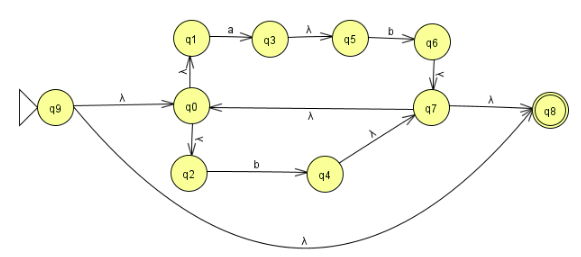
\includegraphics[scale=0.45]{img/letraA.png}
            %\caption{Caption}
            %\label{fig:my_label}
        \end{figure}
        \item Representação do autômato:
            \begin{figure}[H]
            \centering
            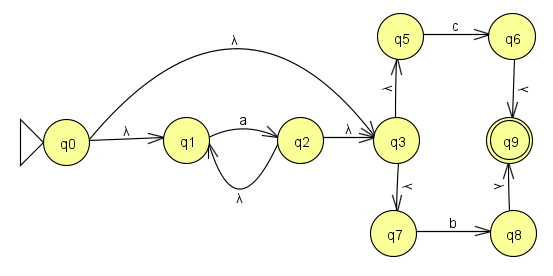
\includegraphics[scale=0.45]{img/letraB.png}
            %\caption{Caption}
            %\label{fig:my_label}
        \end{figure}
    \end{enumerate}
\end{solution}

\begin{problem} Defina a gramática G que gera a linguagem $L = \{w | w$ é palavra de $a(ab)^{*}\}$. Mostre os passos
da derivação para palavra w=aabab.
\end{problem}

\begin{solution} A gramática regular é $G = (\{S,A,B\},\{a,b\},P,S)$, tal que $P$ é: 
\begin{itemize}
    \item S $\Rightarrow$ aA
    \item A $\Rightarrow$ aB $| \epsilon$
    \item B $\Rightarrow$ bA
\end{itemize}
Temos que:
\begin{itemize}
    \item $G =\{V,T,P,S\}$:
\item $V = \{S,A,B\}$
\item $T = \{a,b\}$
\item $P = \{S \Rightarrow aA; A \Rightarrow aB | \epsilon; B \Rightarrow bA\}$
\item $S = \{S\}$
\end{itemize}
Derivação para a palavra $aabab$:
\begin{itemize}
    \item $S \cdots S\rightarrow aA$
    \item $aA \cdots A\rightarrow aB$
    \item $aaB \cdots B\rightarrow bA$
    \item $aabA \cdots A\rightarrow aB$
    \item $aabaB \cdots B\rightarrow bA$
    \item $aababA \cdots A\rightarrow \epsilon$
    \item $aabab$
\end{itemize}
\end{solution}

\begin{problem} Explique com suas palavras o que significa computação no contexto dos autômatos estudados.
\end{problem}

\begin{solution} A computação tenta compreender as definições e propriedades dos modelos matemáticos como as linguagens, os autômatos e as gramáticas. Além disso, a computação estuda as máquinas abstratas com vários modelos, cada um com diferentes habilidades e limitações, a computação é responsável por descrever precisamente o poder computacional de cada máquina.
\end{solution}

\begin{problem} Suponha uma máquina que venda dois tipos de doces, um que custa $R\$0,15$ e outro que custa
$R\$0,20$. Suponha que a máquina aceita somente moedas de $R\$0,05$ e de $R\$0,10$. Suponha,
ainda, que a máquina não dá troco. Faça o autômato finito que modele o funcionamento da
máquina.
\end{problem}

\begin{solution} Representação do autômato:
\begin{center}
\begin{tikzpicture}[scale=0.2]
\tikzstyle{every node}+=[inner sep=0pt]
\draw [black] (15.2,-14.9) circle (3);
\draw (15.2,-14.9) node {$q_0$};
\draw [black] (26,-14.9) circle (3);
\draw (26,-14.9) node {$q_1$};
\draw [black] (36.9,-14.9) circle (3);
\draw (36.9,-14.9) node {$q_2$};
\draw [black] (47.9,-14.9) circle (3);
\draw (47.9,-14.9) node {$q_3$};
\draw [black] (47.9,-14.9) circle (2.4);
\draw [black] (58.6,-14.9) circle (3);
\draw (58.6,-14.9) node {$q_4$};
\draw [black] (58.6,-14.9) circle (2.4);
\draw [black] (6.9,-14.9) -- (12.2,-14.9);
\fill [black] (12.2,-14.9) -- (11.4,-14.4) -- (11.4,-15.4);
\draw [black] (29,-14.9) -- (33.9,-14.9);
\fill [black] (33.9,-14.9) -- (33.1,-14.4) -- (33.1,-15.4);
\draw (31.45,-15.4) node [below] {$5$};
\draw [black] (39.9,-14.9) -- (44.9,-14.9);
\fill [black] (44.9,-14.9) -- (44.1,-14.4) -- (44.1,-15.4);
\draw (42.4,-15.4) node [below] {$5$};
\draw [black] (18.2,-14.9) -- (23,-14.9);
\fill [black] (23,-14.9) -- (22.2,-14.4) -- (22.2,-15.4);
\draw (20.6,-15.4) node [below] {$5$};
\draw [black] (34.935,-17.158) arc (-47.55308:-132.44692:13.165);
\fill [black] (34.94,-17.16) -- (34.01,-17.33) -- (34.68,-18.07);
\draw (26.05,-21.11) node [below] {$10$};
\draw [black] (28.256,-12.93) arc (125.39472:54.60528:15.01);
\fill [black] (45.64,-12.93) -- (45.28,-12.06) -- (44.7,-12.87);
\draw (36.95,-9.66) node [above] {$10$};
\draw [black] (46.577,-12.22) arc (234:-54:2.25);
\draw (47.9,-7.65) node [above] {$10$};
\fill [black] (49.22,-12.22) -- (50.1,-11.87) -- (49.29,-11.28);
\draw [black] (49.223,-17.58) arc (54:-234:2.25);
\draw (47.9,-22.15) node [below] {$5$};
\fill [black] (46.58,-17.58) -- (45.7,-17.93) -- (46.51,-18.52);
\draw [black] (50.9,-14.9) -- (55.6,-14.9);
\fill [black] (55.6,-14.9) -- (54.8,-14.4) -- (54.8,-15.4);
\draw (53.25,-15.4) node [below] {$5$};
\draw [black] (57.277,-12.22) arc (234:-54:2.25);
\draw (58.6,-7.65) node [above] {$10$};
\fill [black] (59.92,-12.22) -- (60.8,-11.87) -- (59.99,-11.28);
\draw [black] (59.923,-17.58) arc (54:-234:2.25);
\draw (58.6,-22.15) node [below] {$5$};
\fill [black] (57.28,-17.58) -- (56.4,-17.93) -- (57.21,-18.52);
\end{tikzpicture}
\end{center}
\end{solution}

\subsection{Avaliação 02 - 2020.1}

    \begin{problem}
        Faça o autômato com pilha que reconheça a linguagem 
        $L = \{ 0^m1^n | m \leq n \}$.Mostre um exemplo de computação incluindo a pilha. 
    \end{problem}
    
    \begin{solution}
        Definindo a gramática em L1, temos a tupla G = (V, T, P, S). Tal que:
        
        \begin{enumerate}[label=]
            \item V: conjunto finito de variáveis ou não-terminais;
            \item T: conjunto finito de símbolos terminais disjunto do conjunto V;
            \item P: conjunto com regras de produção;
            \item S: simbolo inicial distinguido de V;
        \end{enumerate}

        Onde: 
        \begin{enumerate}[label=]
            \item $V = \{S\};$
            \item $T = \{0, 1\};$
            \item $P = \{S \rightarrow \epsilon; S \rightarrow  1; S \rightarrow  0S1; S \rightarrow S1\};$
        \end{enumerate}
        
        O autômato com pilha pode ser definido pela tupla $M = (\Sigma, Q, \Gamma, q_0, F, \Delta)$. Logo em M1, temos: $M1 = (\Sigma, Q, \delta, q_0, \{q_f\}, \Delta)$.
        
       \begin{enumerate}[label=]
            \item $\Sigma = \{0, 1\};$
            \item $Q = \{q_0, q_1, q_f\};$
            \item $\Delta = \{0, 1, S, Z\};$
        \end{enumerate}
        
        Podemos representar o autômato por:
        \begin{figure}[H]
             \centering
             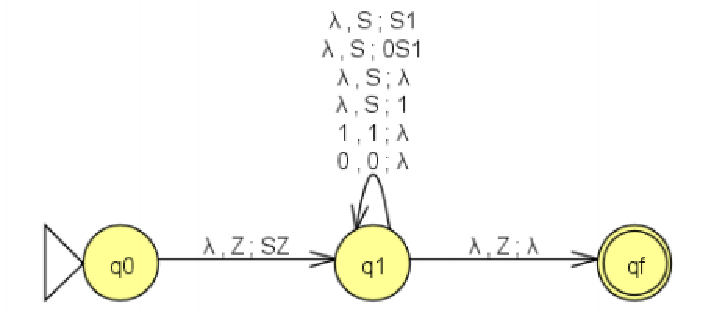
\includegraphics[width=256px]{figs/prova 1/p2f1.pdf}
        \end{figure}
        
    \end{solution}

    \begin{problem}
        Faça o autômato com pilha que reconheça a linguagem que tenha o mesmo número de as e bs. Mostre um exemplo de computação incluindo a pilha.
    \end{problem}
    
    \begin{solution}
        Podemos representar o autômato por:
        \begin{figure}[H]
             \centering
             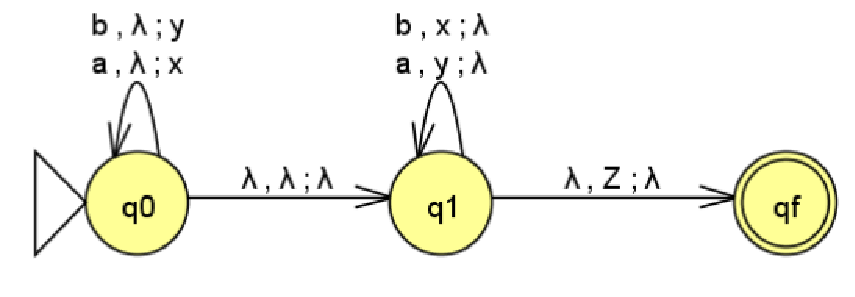
\includegraphics[width=256px]{figs/prova 1/p2f2.pdf}
        \end{figure}

        O autômato com pilha pode ser definido pela tupla $M = (\Sigma, Q, \Gamma, q_0, F, \Delta)$. Logo em M2, temos: $M2 = (\Sigma, Q, \delta, q_0, \{q_f\}, \Delta)$.
        
       \begin{enumerate}[label=]
            \item $\Sigma = \{a, b\};$
            \item $Q = \{q_0, q_1, q_f\};$
            \item $\Delta = \{a, b, x, y, Z\};$
        \end{enumerate}
        
    \end{solution}

    \begin{problem}
        Defina a gramática livre de contexto, incluíndo as regras de produção, que gera $L2 = \{ wcw^R, w \in \{a, b, c\}^* \}$. Mostre a derivação da palavra $w = abcba$. Mostre a árvore de derivação.Existe outra árvore possível? Se sim, mostre pelo menos mais uma árvore. O que significa isso?
    \end{problem}
    
    \begin{solution}
        Definindo a gramática livre de contexto em L2, temos a tupla G2 = (V, T, P, S). Tal que:
        
        \begin{enumerate}[label=]
            \item $V = \{S\};$
            \item $T = \{0, 1\};$
            \item $P = \{S \rightarrow aSa; S \rightarrow  bSb; S \rightarrow  cSc; S \rightarrow c\};$
        \end{enumerate}
        
        Derivando a palavra abcba:
        \begin{itemize}
            \item $S \rightarrow aSa$
            \item $aSa \rightarrow abSba$
            \item $abSba \rightarrow abcba$
        \end{itemize}
        
        A árvore de derivação é definida por: 
        \begin{figure}[H]
             \centering
             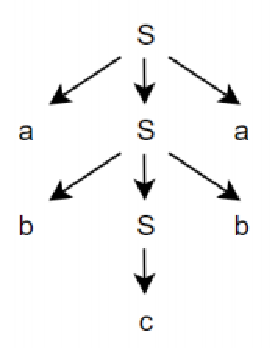
\includegraphics[width=128px]{figs/prova 1/p2f3.pdf}
        \end{figure}
        
        Existe apenas uma árvore de derivação possível. Podemos concluir que a linguagem livre de contexto não é ambígua.
        
        
    \end{solution}
    
    \begin{problem}
        Defina a gramática livre de contexto, incluindo as regras de produção, que gera expressões algébricas com alfabeto $\{x,y,+,-,*,/,(,)\}$. Mostre a derivação da palavra $w = (x+y)^*x / (y-x)^*y$. Mostre a árvore de derivação. Existe outra árvore possível? Se sim, mostre pelo menos mais
        uma árvore. O que significa isso?
    \end{problem}
    
    \begin{solution}
    
        Definindo a gramática livre de contexto, temos a tupla G3 = (V, T, P, S). Tal que: $G3 = (\{S\}, \{x,y,+,-,*,/,(,)\}, P, S)$.
        
        \begin{enumerate}[label=]
            \item $P = \{S \rightarrow S + S;
            S \rightarrow S - S;
            S \rightarrow  S * S; 
            S \rightarrow  S / S;
            S \rightarrow  (S);
            S \rightarrow  x; 
            S \rightarrow  y; 
            \};$
        \end{enumerate}
        
  Derivando a palavra (x+y)*x/(y-x)*y:
        \begin{itemize}
            \item $S \rightarrow S / S$
            \item $S / S \rightarrow S * S / S $
            \item $S * S \rightarrow S * S / S * S$
            \item $S * S / S * S \rightarrow (S) * S / S * S$
            \item $(S) * S / S * S \rightarrow (S) * S / (S) * S$
            \item $(S) * S / (S) * S \rightarrow (S + S) * S / (S)* S $
            \item $ (S + S) * S / (S)* S \rightarrow (S + S) * S / (S - S) * S $
            \item $(S + S) * S / (S - S) * S  \rightarrow (x + S) * S / (S - S) * S $
            \item $(x + S) * S / (S - S) * S  \rightarrow (x + y) * x / (S - S) * S $
            \item $(x + y) * x / (S - S) * S \rightarrow (x + y) * x / (y - S) * S $
            \item $(x + y) * x / (y - S) * S  \rightarrow (x + y) * x / (y - x) * S $
            \item $(x + y) * x / (y - x) * S  \rightarrow (x + y) * x / (y - x) * y $
             
        \end{itemize}
        
        A árvore de derivação é definida por: 
        \begin{figure}[H]
             \centering
             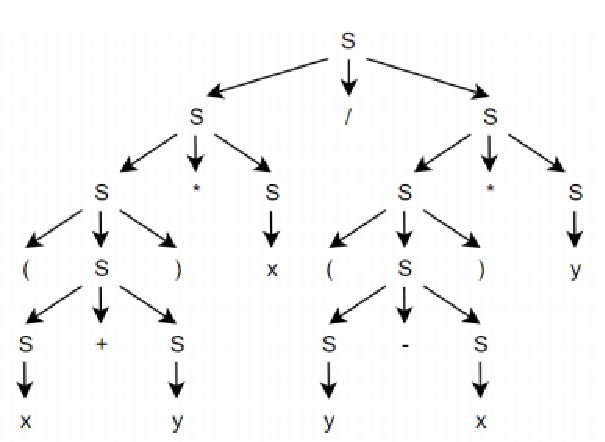
\includegraphics[width=256px]{figs/prova 1/p2f4.pdf}
        \end{figure}
        
        A árvore de derivação não é única, temos também:
        \begin{figure}[H]
             \centering
             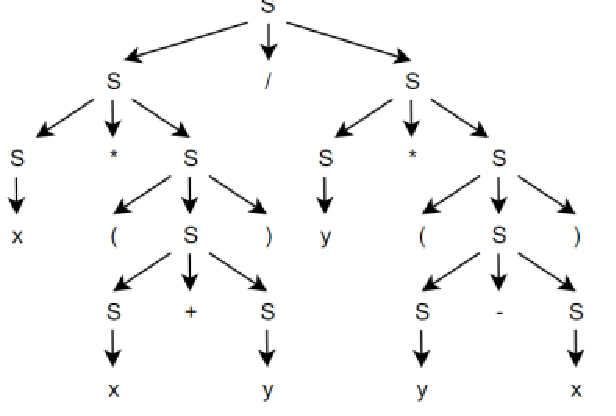
\includegraphics[width=256px]{figs/prova 1/p2f5.pdf}
        \end{figure}
        
        Logo, a gramática livre de contexto é ambígua.
        
    \end{solution}
    
    \begin{problem}
         O que faz a máquina de Turing da Figura 1? Mostre a definição formal e uma computação, incluindo a fita.
         \begin{figure}[H]
             \centering
             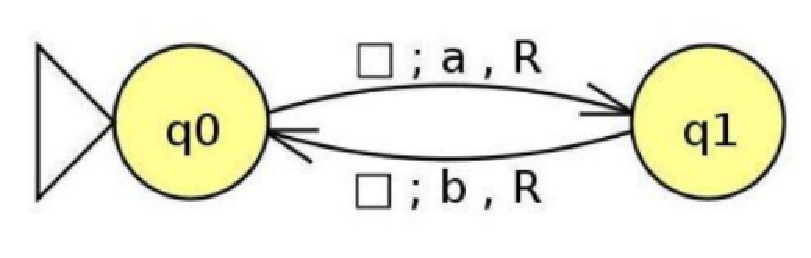
\includegraphics[width=128px]{figs/fig1.pdf}
             \captionsetup{labelformat=empty}
             \caption{Figura 1}
             \label{fig:1}
         \end{figure}
    \end{problem}
    
    \begin{solution}
        A máquina de turing dada escreve palavras com a’s e b’s intercalados.
        
        Pode ser definida formalmente pela tupla: 
        $M = (\{\}, \{q_0, q_1\}, \delta, q_0, \{\}, \{a, b\}, \beta, b)$
        
    \end{solution}
  
    \begin{problem}
          O que faz a máquina de Turing da Figura 2? Mostre a definição formal, a computação da palavra aba, incluindo a fita.
         \begin{figure}[H]
             \centering
             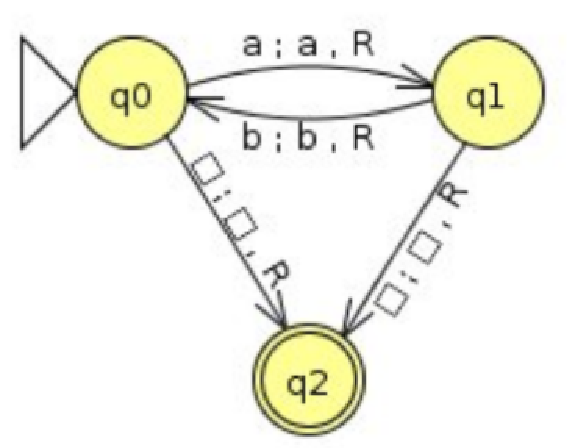
\includegraphics[width=128px]{figs/fig2.pdf}
             \captionsetup{labelformat=empty}
             \caption{Figura 2}
             \label{fig:2}
         \end{figure}
    \end{problem}
    
    \begin{solution}
        A máquina de turing dada aceita palavras vazias, com a ou a’s e bs’s intercalados. Pode ser definida formalmente pela tupla:
        $M = (Q, \Sigma, \delta, q_0, \beta, F)$;
        
        Onde: 
        $M = (\{q_0, q_1, q_2\}, \{a, b\}, \delta, q_0,\beta, \{q_2\})$
        
        Computando a palavra aba:
        \newline
        $\delta(q_0, a) = {(q_1, a, R)}$ \newline
        $\delta(q_1, b) = {(q_0, b, R)}$ \newline
        $\delta(q_0, a) = {(q_1, a, R)}$ \newline
        $\delta(q_1, \beta) = {(q_2, \beta, R)}$
        
        \begin{figure}[H]
             \centering
             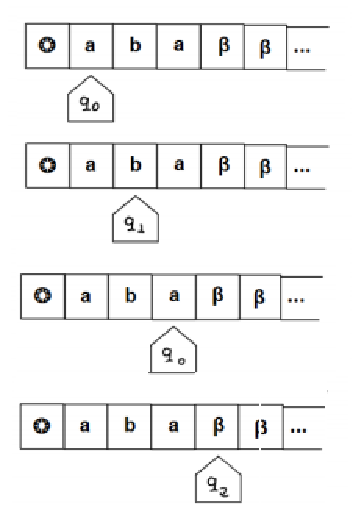
\includegraphics[width=128px]{figs/prova 1/p2f8.pdf}
        \end{figure}
         
    \end{solution}
    
    \begin{problem}
         Faça a máquina de Turing que reconheça palavras na linguagem $L=00^*$, onde $\sum = \{0,1\}$. 
    \end{problem}
    
    \begin{solution}
        
        A máquina de turing pode ser definida pela tupla:\newline
        $M = (\{0, 1\}, \{q_0, q_1, q_f\}, \delta, q_0, \{q_f\}, \{0\}, \beta, b)$
        
        \begin{figure}[H]
             \centering
             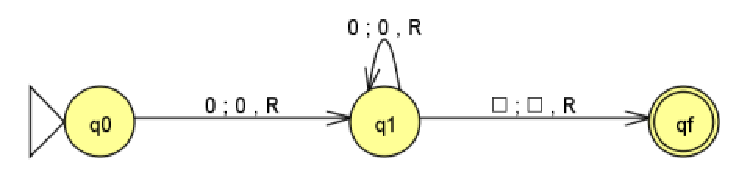
\includegraphics[width=252px]{figs/prova 1/p2f9.pdf}
        \end{figure}
    \end{solution}
    
    \begin{problem}
        Faça a máquina de Turing que realize soma de números representados por quantidade de uns. Por exemplo, 2=11, 5=11111, etc. Os dois operandos são separados por um zero.
        Exemplo: 2+3=110111=11111.
    \end{problem}
    
    
    \begin{solution}
        O autômato pode ser definido pela tupla:\newline
        $M = (\{0, 1\}, \{q_0, q_1, q_2, q_3, q_4\}, \delta, q_0, \{q_4\}, \{1\}, \beta, b)$.
        
        Assim, temos o autômato:
        
        \begin{figure}[H]
             \centering
             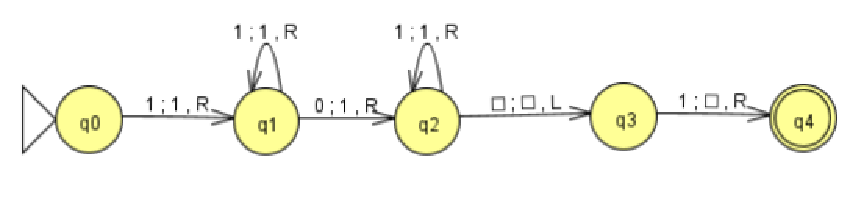
\includegraphics[width=256px]{figs/prova 1/p2f6.pdf}
         \end{figure}
    \end{solution}
    
    \begin{problem}
         Explique a diferença entre:
            \begin{enumerate}[label=(\alph*)]
            \item Gramática irrestrita e gramática sensível ao contexto;
            \item Máquina de Turing como reconhecedor de linguagens recursivamente enumeráveis e de linguagens sensíveis ao contexto.
            \end{enumerate}
    \end{problem}
    
    \begin{solution}
        \begin{enumerate}[label=(\alph*)]
            \item A gramática irrestrita gera o conjunto das linguagens recursivamente enumeráveis, logo suas regras de produção não
            possuem restrições. O formalismo reconhecedor equivalente à
            gramática irrestrita é a Máquina de Turing. - A gramática sensível
            ao contexto gera o conjunto das linguagens sensíveis ao contexto,
            suas regras de produção possuem restrições e essas restrições
            estão ligadas a um contexto, este pode ser definido como um
            elemento associado ao domínio das regras de produção que possui
            mais de um elemento em conjunto, podendo ser uma sequência de
            variáveis e/ou terminais que possuem derivações de tamanho maior
            ou igual a esta sequência. O formalismo reconhecedor equivalente à
            gramática sensível ao contexto é a Máquina de Turing com fita
            limitada.
            
            \item A principal diferença entre as duas ocorre no fato de que para uma Linguagem
            Recursivamente Enumerável a fita é ilimitada, enquanto que para uma Linguagem Sensível
            ao Contexto ela possui restrição no limite de sua fita. Além disso, a LRE é gerada por uma
            gramática Irrestrita e tem 3 destinos possíveis: parar e aceitar a palavra, parar e recusar a
            palavra ou entrar em um loop infinito, no qual não será possível dizer se a palavra é aceita
            ou não. A Linguagem Sensível ao Contexto está contida na Linguagem Recursivamente
            Enumerável e, como já dito anteriormente, tem tamanho limitado e sempre irá parar,
            aceitando ou rejeitando a palavra
        \end{enumerate}
    \end{solution}

\end{document}